\documentclass[t,serif]{beamer}
\usepackage[portuguese,brazil]{babel} % nomes em portugues
\usepackage[utf8]{inputenc} % acentuacao
\usepackage[T1]{fontenc}
\usepackage{ae} % separacao de sílabas de palavras com acento
\usepackage{icomma}         % acerta espacamento quando a vi­rgula
\usepackage{color}
\usepackage{enumerate}
\usepackage{courier}

\usetheme{Boadilla}
% \usetheme{Copenhagen}
%\usetheme{default}
%\usecolortheme{beaver}
\usecolortheme{seahorse}
\usepackage{textpos}

%%% 1) General Comands
\newcommand{\abf}{\mathbf{a}}
\newcommand{\corr}{\color{red}}
\newcommand{\corb}{\color{blue}}
\newcommand{\corg}{\color{green}}
\newcommand{\cork}{\color{black}}
\newcommand{\cory}{\color{gray}}
\newcommand{\TitleSlide}[1]{\begin{frame} \centering #1 \end{frame}}

% Important constants
\newcommand{\oobf}{\boldsymbol{\o}}
\newcommand{\pibf}{\boldsymbol{\pi}}
\newcommand{\varpibf}{\boldsymbol{\varpi}}

%%% 6) Some operators
\newcommand{\EV}{{\rm E}}          % Expected Value
\newcommand{\TR}{{\rm tr}}         % Trace

\newcommand{\sen}{\textrm{sen}}
\renewcommand{\cos}{\textrm{cos}}
\newcommand{\e}{\textrm{e}}
\newcommand{\cotg}{\textrm{cotg}}
\newcommand{\cosec}{\textrm{cosec}}

\title[GitHub Actions]{\textbf{\underline{GitHub Actions}}}
\subtitle{{\small Tópicos Especiais em Sistemas de Energia Elétrica II: Desenvolvimento Ágil com Python e Containers\\Prof. Angelo Colombini}}
\author[Rene Cruz Freire]{Rene Cruz Freire}
\date{renefreire@id.uff.br}
\institute[]{Universidade Federal Fluminense\\Campus Niterói}

\setbeamertemplate{blocks}[rounded][shadow=true]
%\setbeamertemplate{footline}[frame number]  %Apaga a linha inferior com o nome do professor
%\setbeamertemplate{page number in head/foot}[totalframenumber]

\begin{document}

% Capa
\frame{
	\vspace*{-0.2cm}
\includegraphics[height=2.8cm]{figs/escola_eng.png}\hspace*{3.5cm}
\includegraphics[height=2.8cm]{figs/ppgeet.jpeg}
	\titlepage
}

\addtobeamertemplate{frametitle}{}{%
	\begin{textblock*}{100mm}(.78\textwidth,-1cm)
		\hspace{1.0cm}
\includegraphics[height=1cm]{figs/logo_uff.png}
	\end{textblock*}
}

% Sumário
\section*{Sumário}
	\begin{frame}{Sumário}
		\scriptsize
		\tableofcontents%[pausesections]
	\end{frame}

\section{Visão Geral}
	% Slide 03
	\begin{frame}{Visão Geral}
		\vspace{0.5cm}
		\begin{itemize}
			\item O GitHub Actions é uma plataforma de integração e entrega/deployment contínuos (CI/CD), que automatiza os \textit{workflows} de desenvolvimento de software.
			\vspace{0.5cm}
			\item Ele permite que você crie, teste e faça \textit{deploy} de um código-fonte de software diretamente do seu repositório GitHub, criando fluxos de trabalho ou \textit{pipelines} personalizados.
			\vspace{0.5cm}
			\item Com várias opções de configuração para gatilhos baseados em \textit{commits} e \textit{merges}, o GitHub Actions é uma boa escolha para fluxos de trabalho baseados em GitOps.
		\end{itemize}
	\end{frame}
	
\section{Funcionamento}
	% Slide 04
	\begin{frame}{Funcionamento}
		\vspace{0.5cm}
		\begin{itemize}
			\item Os fluxos de trabalho do GitHub Actions são configurados usando arquivos YAML, que definem a sequência de tarefas ou ações a serem executadas quando acionadas por eventos como \textit{pushes}, \textit{pull requests} e \textit{releases} de código.
			\vspace{0.5cm}
			\item Ações são blocos reutilizáveis de código que executam tarefas específicas, como configurar dependências, executar testes e fazer o \textit{deploy} em um provedor de nuvem ou servidores locais.
			\vspace{0.5cm}
			\item É possível criar e publicar ações personalizadas para suas necessidades específicas.
		\end{itemize}
	\end{frame}
	
	% Slide 05
	\begin{frame}{Funcionamento}
		\vspace{0.5cm}
		\begin{itemize}
			\item O GitHub fornece máquinas virtuais, também conhecidas como \textit{runners}, para executar seus fluxos de trabalho em ambientes Linux, Windows e macOS.
			\vspace{0.5cm}
			\item Os \textit{runners} oferecem suporte a qualquer linguagem de programação, plataforma e provedor de nuvem, tornando o GitHub flexível para vários projetos.
			\vspace{0.5cm}
			\item O GitHub Actions integra-se perfeitamente com outros recursos do GitHub, como as \textit{issues}, \textit{pull requests} e \textit{marketplace}, permitindo a criação de fluxos de trabalho automatizados com base em eventos no seu repositório.
		\end{itemize}
	\end{frame}
	
	% Slide 06
	\begin{frame}{Funcionamento}
		\begin{center}
			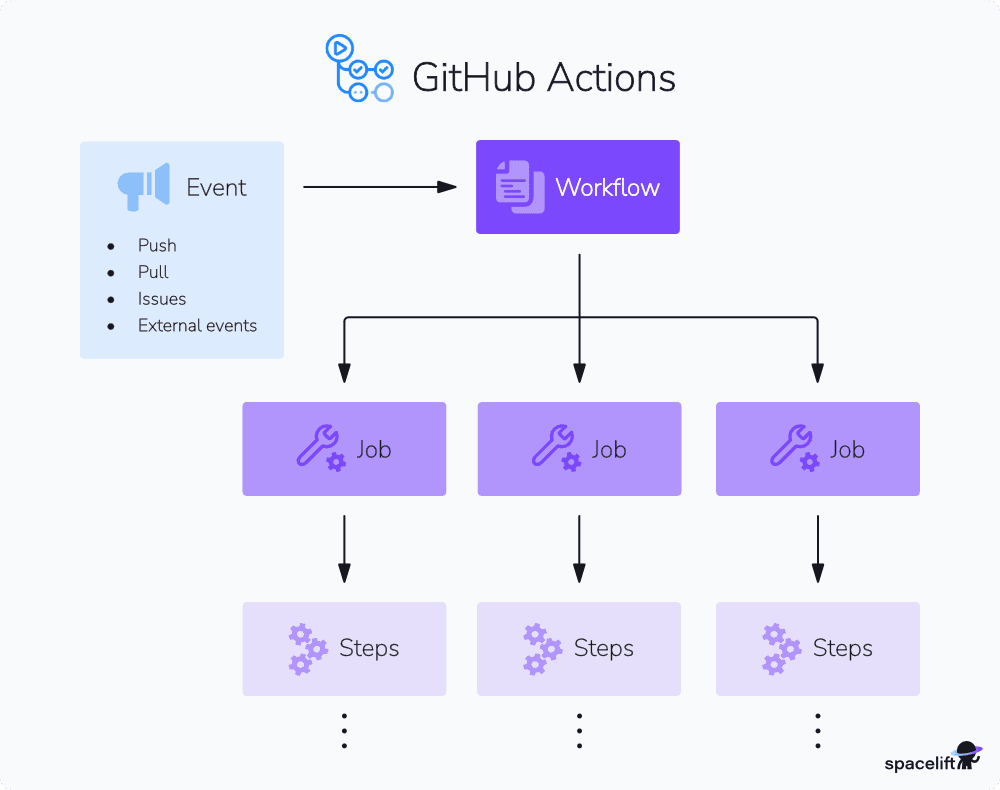
\includegraphics[width=0.8\linewidth]{figs/3_1.png}
		\end{center}
	\end{frame}
	
\section{Curva de Aprendizado}
	% Slide 07
	\begin{frame}{Curva de Aprendizado}
		\vspace{0.5cm}
		\begin{itemize}
			\item O GitHub Actions geralmente é considerado fácil de aprender, especialmente para desenvolvedores já familiarizados com o GitHub e conceitos básicos de \textit{script}.
			\vspace{0.5cm}
			\item Ele fornece um ponto de entrada fácil de usar para automação, permitindo que os desenvolvedores configurem rapidamente pipelines básicos de CI/CD e outros fluxos de trabalho sem amplo conhecimento de DevOps.
			\vspace{0.5cm}
			\item Como acontece com qualquer ferramenta, dominar recursos mais avançados e casos de uso complexos exigirá mais tempo e prática.
		\end{itemize}
	\end{frame}
	
\section{Componentes}
	% Slide 08
	\begin{frame}{Componentes}
		\vspace{0.5cm}
		\begin{itemize}
			\item É possível configurar um fluxo de trabalho do GitHub Actions a ser disparado quando um evento ocorrer no seu repositório, como a abertura de uma solicitação de pull ou a criação de um problema.
			\vspace{0.5cm}
			\item Um fluxo de trabalho contém um ou mais \textit{jobs} que podem ser executados em ordem sequencial ou em paralelo.
			\vspace{0.5cm}
			\item Cada \textit{job} será executado em um \textit{runner} próprio ou em um contêiner, e tem uma ou mais etapas que executam um \textit{script} definido pelo usuário ou uma ação, que é uma extensão reutilizável que pode simplificar o fluxo de trabalho.
		\end{itemize}
	\end{frame}
	
	% Slide 09
	\begin{frame}{Componentes}
		\begin{enumerate}
			\item[1.] \textbf{\textit{Workflow}}: é um processo automatizado definido por um arquivo YAML.
			\item[2.] \textbf{Eventos}: são atividades específicas que acionam a execução de um fluxo de trabalho.
			\item[3.] \textbf{\textit{Runners}}: são máquinas virtuais que executam \textit{jobs} em um fluxo de trabalho.
			\item[4.] \textbf{\textit{Job}}: consiste em uma série de etapas executadas, em paralelo ou sequencialmente, no mesmo \textit{runner}.
			\item[5.] \textbf{\textit{Steps}}: são as tarefas ou comandos individuais que compõem um \textit{job}.
			\item[6.] \textbf{Ações}: são pacotes de código reutilizáveis usados como etapas em um fluxo de trabalho.
		\end{enumerate}
	\end{frame}
	
	% Slide 10
	\begin{frame}{Componentes}
		\begin{center}
			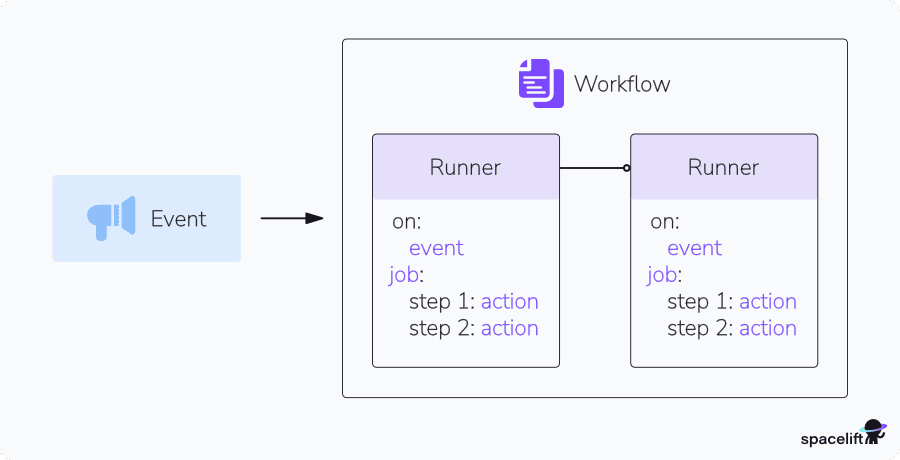
\includegraphics[width=\linewidth]{figs/3_2.png}
		\end{center}
	\end{frame}
	
\section{Vantagens e Desvantagens}
	% Slide 11
	\begin{frame}{Vantagens e Desvantagens}
		\textbf{Vantagens}
		\begin{enumerate}
			\item[1.] \textbf{Integração nativa com o GitHub}: Totalmente integrado ao ecossistema GitHub, o que facilita o uso e evita ferramentas externas para automação.
			\item[2.] \textbf{Fácil de começar}: Com poucos cliques ou arquivos YAML simples, já é possível criar \textit{workflows} de CI/CD rapidamente.
			\item[3.] \textbf{Gratuito para projetos públicos}: Repositórios públicos têm acesso ilimitado aos \textit{runners} hospedados pela plataforma.
			\item[4.] \textbf{Flexibilidade de \textit{workflows}}: Suporta múltiplos gatilhos (\textit{push}, \textit{pull request}, \textit{cron}, \textit{release}, etc.) e etapas condicionais, possibilitando pipelines altamente personalizados.
			\item[5.] \textbf{Suporte a containers e ambientes personalizados}: Pode rodar \textit{job}s em containers Docker ou em VMs \textit{self-hosted}, aumentando a flexibilidade do ambiente de \textit{build}.
		\end{enumerate}
	\end{frame}
	
	% Slide 12
	\begin{frame}{Vantagens e Desvantagens}
		\textbf{Desvantagens}
		\begin{enumerate}
			\item[1.] \textbf{Limitações no plano gratuito para repositórios privados}: Existe um limite de minutos e armazenamento para repositórios privados, especialmente em contas gratuitas.
			\item[2.] \textbf{Performance e tempo de espera}: Em horários de pico ou em contas gratuitas, os runners hospedados podem ter filas ou performance inferior.
			\item[3.] \textbf{Limitações nos logs}: Os logs podem ser truncados ou difíceis de depurar quando há muitos \textit{steps} ou \textit{jobs} em execução.
			\item[4.] \textbf{Menos controle sobre infraestrutura dos runners hospedados}: Comparado a soluções como Jenkins em ambiente próprio, há menos controle sobre a configuração do ambiente.
			\item[5.] \textbf{Falta de UI mais avançada para workflows complexos}: A interface do GitHub Actions ainda é relativamente simples para pipelines muito grandes ou com múltiplos caminhos condicionais.
		\end{enumerate}
	\end{frame}
	
\section{Primeiro \textit{Workflow} no GitHub Actions}
	% Slide 11
	\begin{frame}{Primeiro \textit{Workflow} no GitHub Actions}
		\textbf{Pré-requisitos}
		\begin{itemize}
			\item É necessário um conhecimento básico do GitHub.
			\item Deve-se ter um repositório no GitHub para adicionar os arquivos.
			\item Deve-se ter acesso ao GitHub Actions.
		\end{itemize}
		\begin{block}{Observações:}
			\begin{itemize}
				\item Se a aba \textbf{Actions} não for exibida sob o nome do seu repositório, tal como na figura a seguir, provavelmente o Actions está desabilitado para o repositório.
			\end{itemize}
			\begin{center}
				
\includegraphics[width=0.9\linewidth]{figs/3_3.png}
			\end{center}
		\end{block}
	\end{frame}
	
	% Slide 12
	\begin{frame}{Primeiro \textit{Workflow} no GitHub Actions}
		\begin{enumerate}
			\item[1.] No seu repositório no GitHub, crie um arquivo de \textit{workflow} chamado \texttt{github-actions-demo.yml} no diretório \texttt{.github/workflows}.
			\vspace{0.2cm}
			\begin{itemize}
				\item Se o diretório \texttt{.github/workflows} já existir, navegue até ele no GitHub, clique em adicionar arquivo, depois clique em criar novo arquivo e nomeie o arquivo como \texttt{github-actions-demo.yml}.
				\vspace{0.2cm}
				\item Se o seu repositório não tiver um diretório \texttt{.github/workflows}, vá para a página principal do repositório no GitHub, clique em adicionar arquivo, depois clique em criar novo arquivo e nomeie o arquivo \texttt{.github/workflows/github-actions-demo.yml}.
				\begin{itemize}
					\item Isso cria os diretórios \texttt{.github} e \texttt{workflows} e o arquivo \texttt{github-actions-demo.yml} em uma única etapa.
				\end{itemize}
			\end{itemize}
		\end{enumerate}
	\end{frame}
	
	% Slide 13
	\begin{frame}{Primeiro \textit{Workflow} no GitHub Actions}
		\vspace{1cm}
		\begin{block}{Observações:}
			\begin{itemize}
				\item Para que o GitHub descubra quaisquer fluxos de trabalho do GitHub Actions no seu repositório, você deve salvar os arquivos de \textit{workflow} em um diretório chamado \texttt{.github/workflows}.
				\item É possível dar ao arquivo de fluxo de trabalho o nome que desejar, mas deve-se usar \texttt{.yml} ou \texttt{.yaml} como extensão do nome do arquivo.
				\item YAML é uma linguagem de marcação comumente usada para arquivos de configuração.
			\end{itemize}
		\end{block}
	\end{frame}
	
	% Slide 14
	\begin{frame}{Primeiro \textit{Workflow} no GitHub Actions}
		\begin{enumerate}
			\item[2.] Escreva o seguinte conteúdo no arquivo \texttt{.yml}:
			\begin{center}
				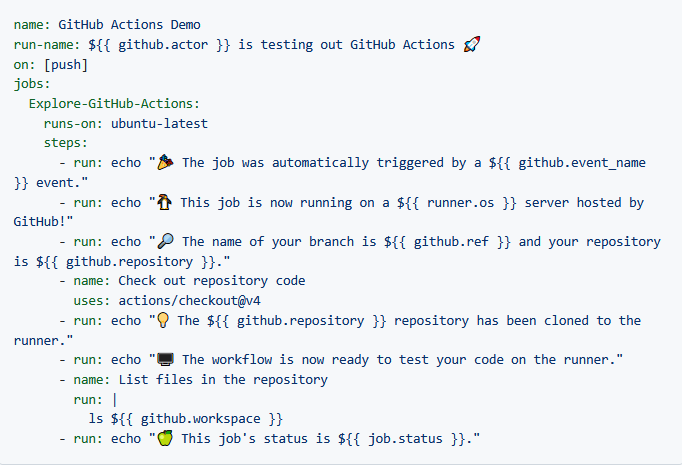
\includegraphics[width=0.9\linewidth]{figs/3_4.png}
			\end{center}
		\end{enumerate}
	\end{frame}
	
	% Slide 15
	\begin{frame}{Primeiro \textit{Workflow} no GitHub Actions}
		\begin{columns}
			\column{0.5\linewidth}
				\\
				\begin{enumerate}
					\item[3.] Clique em \textbf{commit changes}
					\item[4.] Na caixa de diálogo \textbf{Propose changes}, selecione a opção de confirmar a \textit{branch} padrão ou a opção de criar uma nova \textit{branch} e iniciar um \textit{pull request}, e em seguida clique em \textit{commit changes} ou \textit{propose changes}.
				\end{enumerate}
			\column{0.5\linewidth}
				\\
				\begin{center}
					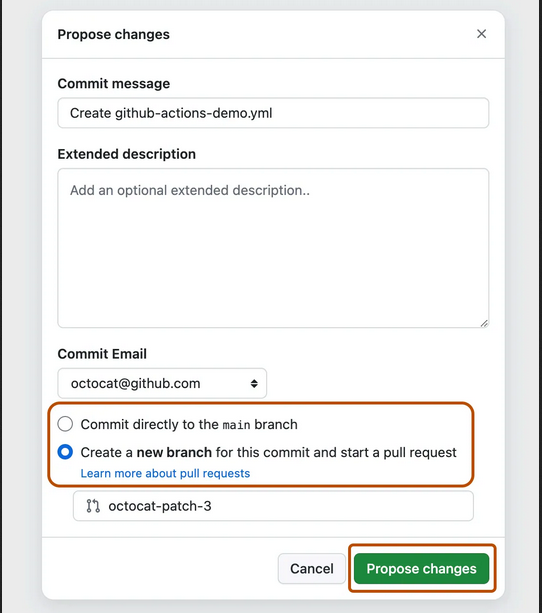
\includegraphics[width=\linewidth]{figs/3_5.png}
				\end{center}
		\end{columns}
	\end{frame}
	
	% Slide 16
	\begin{frame}{Primeiro \textit{Workflow} no GitHub Actions}
		\vspace{1cm}
		\begin{block}{Observações:}
			\begin{itemize}
				\item Enviar o arquivo de fluxo de trabalho para uma ramificação no seu repositório aciona o evento push e executa seu fluxo de trabalho.
				\item Se você optar por iniciar uma solicitação de pull, poderá continuar e criá-la, mas isso não é necessário para os propósitos deste início rápido porque a confirmação ainda foi feita em uma ramificação e acionará o novo fluxo de trabalho.
			\end{itemize}
		\end{block}
	\end{frame}
	
\section{Visualizando os Resultados do \textit{Workflow}}
	% Slide 17
	\begin{frame}{Visualizando os Resultados do \textit{Workflow}}
		\begin{enumerate}
			\item[1.] No GitHub, navegue até a página principal do repositório.
			\item[2.] Abaixo do nome do repositório, clique em \textbf{Actions}.
			\begin{center}
				
\includegraphics[width=\linewidth]{figs/3_6.png}
			\end{center}
			\item[3.] Na barra lateral esquerda, clique no fluxo de trabalho que deseja exibir, neste exemplo "GitHub Actions Demo".
			\begin{center}
				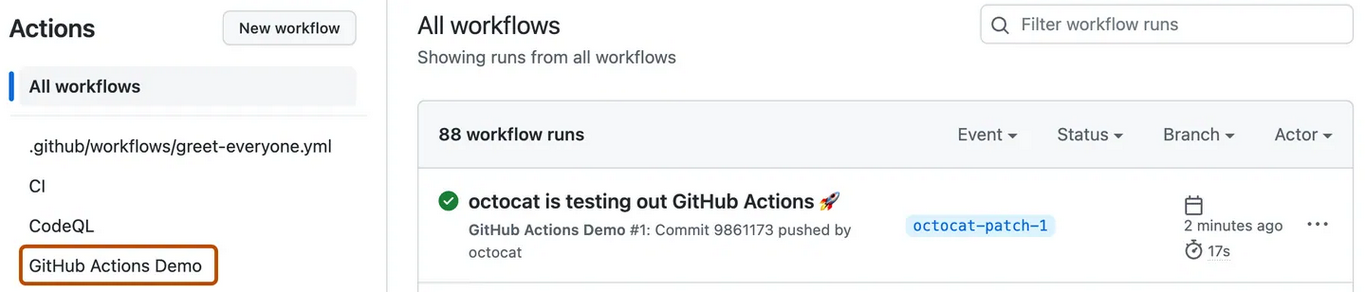
\includegraphics[width=\linewidth]{figs/3_7.png}
			\end{center}
		\end{enumerate}
	\end{frame}
	
	% Slide 18
	\begin{frame}{Visualizando os Resultados do \textit{Workflow}}
		\begin{enumerate}
			\item[4.] Na lista de execuções de fluxo de trabalho, clique no nome da execução que deseja ver. Neste exemplo, "USERNAME is testing out GitHub Actions".
			\item[5.] Na barra lateral esquerda da página de execução do \textit{workflow}, em \texttt{Jobs}, clique em \texttt{Explore-GitHub-Actions}.
			\begin{center}
				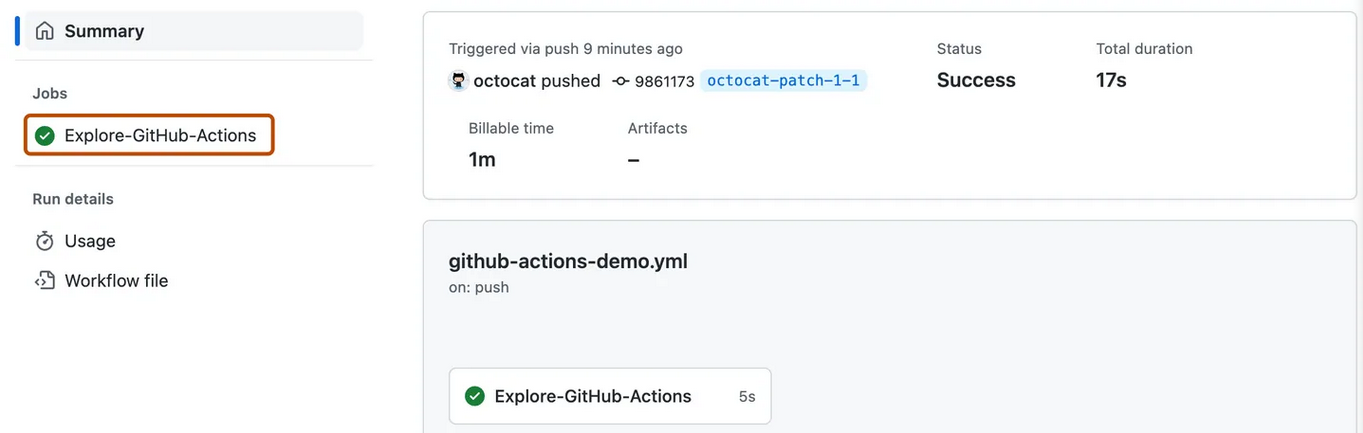
\includegraphics[width=\linewidth]{figs/3_8.png}
			\end{center}
		\end{enumerate}
	\end{frame}
	
	% Slide 19
	\begin{frame}{Visualizando os Resultados do \textit{Workflow}}
		\begin{enumerate}
			\item[6.] O log mostra como cada etapa foi processada. Expanda qualquer uma das etapas para ver seus detalhes.
			\begin{center}
				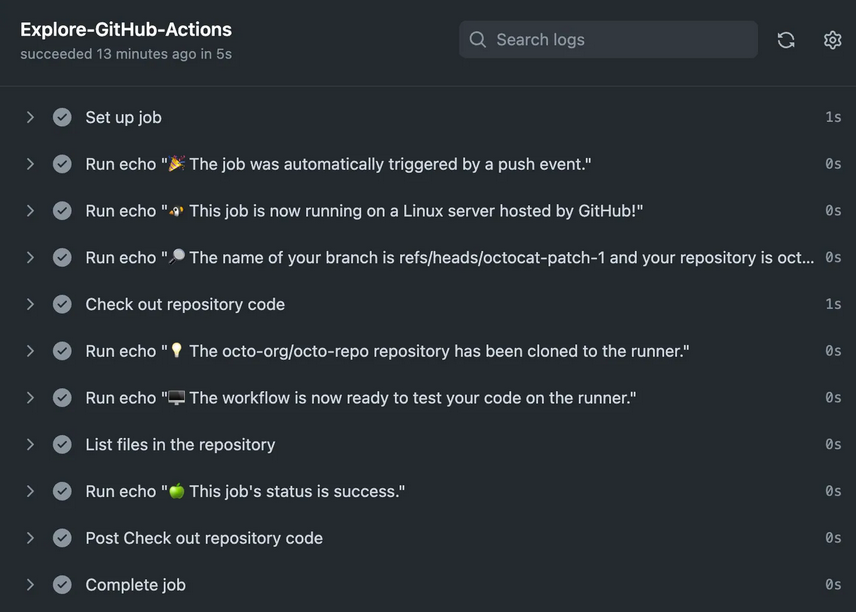
\includegraphics[width=0.8\linewidth]{figs/3_9.png}
			\end{center}
		\end{enumerate}
	\end{frame}
	
\section{Referências}
	% Slide 20
	\begin{frame}{Referências}
		\begin{itemize}
			\item https://docs.github.com/en/actions/writing-workflows/quickstart - Inicializando um \textit{workflow no GitHub Actions}.
			\item https://docs.github.com/en/actions/about-github-actions/understanding-github-actions - Visão geral sobre o GitHub Actions.
			\item https://docs.github.com/en/actions/writing-workflows/about-workflows\#understanding-the-workflow-file - Aprofundamento sobre os \textit{workflows no GitHub Actions}
			\item https://docs.github.com/en/enterprise-cloud@latest/actions/guides - Listagem de guias sobre o GitHub Actions
			\item https://spacelift.io/blog/github-actions-tutorial - Tutorial sobre o GitHub Actions
		\end{itemize}
	\end{frame}
\end{document}
